\documentclass{article}

\usepackage{amsmath}

\usepackage{xtab}

\usepackage{graphicx}

\usepackage{subfigure}

\usepackage{fullpage}

\usepackage{hyperref}

\usepackage{amsmath}


\author{Marcela De La Cruz}

\date{\today}



\title{\sc Teor\'ia b\'asica de flujo}

\pagestyle{empty}



\begin{document}

\maketitle 

\thispagestyle{empty}  

\section{Definici\'on de permeabilidad} % (fold)

\label{sec:definicion}


La permeabilidad es la unidad de medida de la facilidad de flujo de un fluido (incluso un gas) a trav\'es de un medio poroso.

Se afirma que un material es permeable si deja pasar a trav\'es de \'el una cantidad apreciable de fluido en un tiempo dado, e impermeable si la cantidad de fluido es despreciable.


La velociead con la que el fluido atraviesa el material depende de tres factores b\'asicos:


\begin{itemize}

\item{La porosidad del material}

\item{La densidad del fluido considerado, afectado por la temperatura} 

\item{La presi\'on a que est\'a sometido el fluido}

\end{itemize}


Para ser permeable, un material debe ser poroso, es decir, debe contener espacios vac\'ios o poros que le permitan absorber fluido. A su vez, tales espacios deben estar interconectados para que el fluido disponga de caminos para pasar a trav\'es del material. Un ejemplo de roca porosa se muestra en la figura \ref{fig:poros}


\begin{figure}[h]

\centering

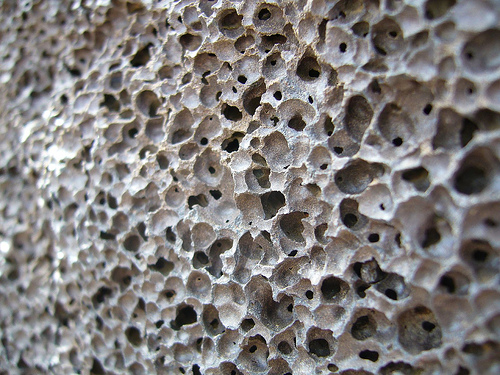
\includegraphics[width=0.5\textwidth]{poros}

\caption{Roca porosa}

\label{fig:poros}

\end{figure}


% section definición_de_permeabilidad (end)


\section{Determinaci\'on de la permeabilidad} % (fold)

\label{sec:form}


La permeabilidad de cualquier material poroso, se determina mediante la f\'ormula de Darcy:

\begin{equation}
{K} = \frac{Q\mu L}{A(P_{1}-P_{2})} 
\end{equation}


% section form (end)

\section{Tipos de permeabilidad} % (fold)

\label{sec:tipos}
\begin{center}
\begin{tabular}{|p{0.15\textwidth}|p{0.80\textwidth}|}

\hline
\textbf{Porosidad} & \textbf{Definici\'on}\\
\hline
\hline

Absoluta  & Es la conductividad de una roca o material poroso cuando est\'a saturado completamente por un solo fluido.\\
Efectiva  & Es la conductividad de un material poroso a una fase cuando dos o m\'as fases est\'an presentes y tambi\'en se mide en Darcy. Cuando dos o m\'as
            fases est\'an fluyendo simult\'aneamente en un medio poroso permeable, como por ejemplo en un proceso de desplazamiento, la permeabilidad efectiva
             a una fase dada es menor que la permeabilidad absoluta y es funci\'on de la saturaci\'on de la fase.\\
Relativa  & Es la raz\'on entre la permeabilidad efectiva y una permeabilidad base.\\

\hline

\end{tabular}
\end{center}
% section tipos (end)



\end{document}